\documentclass[10pt,b5paper,titlepage]{book}

\usepackage[utf8]{inputenc}
\usepackage{amsmath}
\usepackage{amsfonts}
\usepackage{amssymb}
%\usepackage{xcolor}
\usepackage{color}
\usepackage{graphicx}

\usepackage{hyperref}

\author{Jan Tomek}
\title{\bf Matrix Algebra}

\setlength{\parindent}{0ex}
\renewcommand{\labelitemi}{$\bullet$}
\renewcommand{\labelitemii}{$\bullet$}
\renewcommand{\labelitemiii}{$\bullet$}
\renewcommand{\labelitemiv}{$\bullet$}

%Commands definitions
\newcommand\setbackgroundcolour{\pagecolor[rgb]{0.15,0.15,0.15}}
\newcommand\settextcolour{\color[rgb]{0.9,0.9,0.9}}
\newcommand\invertbackgroundtext{\setbackgroundcolour\settextcolour}

% {name}[number of arguments][1st default value] etc..
% the argument value is then inserted at #argument_number
\newenvironment{bbox}[1][1.0]
{
    \begin{center}
        \begin{tabular}{|p{#1\textwidth}|}
            \hline\\
}
{
            \\\\\hline
        \end{tabular}
    \end{center}
}

\newenvironment{bboxtitle}[1][1.0]
{
    \begin{center}
        #1\\[1ex]
        \begin{tabular}{|p{#1\textwidth}|}
            \hline\\
}
{
            \\\\\hline
        \end{tabular}
    \end{center}
}

%Command execution.
%If this line is commented, then the appearance remains as usual.
\invertbackgroundtext


\begin{document}

\maketitle

\tableofcontents

\chapter{Inner Product Space}

From: \url{http://fourier.eng.hmc.edu/e176/lectures/algebra/node1.html}\\

\begin{itemize}
    \item \textbf{Vector space}\\

        A \textit{vector space} over a field $F$ is a set $V$ which closed under
        the following two operations of addition and scalar multiplication
        defined for its members (called \textit{vectors}), i.e., the results
        of the operations are also members of $V$.

        \begin{enumerate}
            \item The vector addition that maps any two vectors
                $\mathbf{x}, \mathbf{y} \in V$ to another vector
                $\mathbf{x} + \mathbf{y} \in V$ satisfiying the following
                properties:
                \begin{itemize}
                    \item Commutativity: $\mathbf{x} + \mathbf{y} = \mathbf{y} + \mathbf{x}$.
                    \item Associativity: $\mathbf{x} + (\mathbf{y} + \mathbf{z}) = (\mathbf{x} + \mathbf{y}) + \mathbf{z}$.
                    \item Existence of zero: there is a vector $\mathbf{0} \in V$ such that: $\mathbf{0} + \mathbf{x} = \mathbf{x} + \mathbf{0} = \mathbf{x}$.
                    \item Existence of inverse: for any vector $\mathbf{x} \in V$,
                        there is another vector $-\mathbf{x} \in V$ such that $\mathbf{x} + (- \mathbf{x}) = \mathbf{0}$.
                \end{itemize}
            \item The scalar multiplication that maps a vector $\mathbf{x \in V}$
                and scalar $a \in F$ ($F$ can be a real or complex fiels) to another
                vector $a \mathbf{x} \in V$ with the following properties:

                \begin{itemize}
                    \item $a (\mathbf{x} + \mathbf{y} = a \mathbf{x} + a \mathbf{y}$.
                    \item $(a + b) \mathbf{x} = a \mathbf{x} + b \mathbf{x}$.
                    \item $a b \mathbf{x} = a (b \mathbf{x})$.
                    \item $\mathbf{1} \mathbf{x} = \mathbf{x}$.
                \end{itemize}
        \end{enumerate}

        where $\mathbf{0} = [0, \ldots, 0]^{T}$ and $\mathbf{1} = [1, \ldots, 1]^{T}$
        are two constant vectors.\\

        A subset $W$ of $V$ is a subspace of $V$, denoted by $W \subseteq V$,
        if it is also a vector space, i.e., it is closed under the same
        operations defined in $V$:

        \begin{enumerate}
            \item The zero vector $\mathbf{0}$ of $V$ must be in $W$
                (the zero vector is unique in $V$, which $W$ must have).
            \item For any $\mathbf{x}, \mathbf{y} \in W, \mathbf{x} + \mathbf{y} \in W$.
            \item For any $\mathbf{x} \in W, a \mathbf{x} \in W$.
        \end{enumerate}

        Listed below is a set of typical vector spaces:

        \begin{itemize}
            \item $n$-D vector space $\mathbb{R}^{n}$ or $\mathbb{C}^{n}$

                This space contains all $n$-D vectors expressed as an  $n$-tuple,
                an ordered list of $n$ elements (or components):

                \begin{equation}
                    \mathbf{x} = \begin{bmatrix} x_1\\ x_2 \\ \vdots\\ x_n \end{bmatrix} =
                    \begin{bmatrix} x_1 & \ldots & x_n \end{bmatrix}^{T}
                ,\end{equation}

                which can be used to represent a discrete signal containing
                $n$ samples. We will always represent a vector as a vertical
                or column vector, or the transpose of a horizontal or row
                vector. The space is denoted by either $\mathbb{C}^{n}$ if the elements
                are complex $x_{i} \in \mathbb{C}$, or $\mathbb{R}^{n}$ if they
                are real $x_{i} \in \mathbb{R} (i = 1, \ldots, n)$.

                A subspace of $\mathbb{R}^{n}$ can be a $\mathbb{R}^{m} (m < n)$
                that passes origin (zero). For example, any 2-D plane passing
                through the origin of a 3-D space is its subspace. However, if
                the 2-D plane does not pass through the origin, it is not a subspace.
                Also, as 3-D cube or sphere centered at the origin is not a subspace,
                as it is not closed under the operations of addition and scalar
                multiplication.

            \item A vector space can be defined to contain all $m \times n$ matrices
                composed of $n$ $m$-D column vectors:

                \begin{equation}
                    \mathbf{A} = \begin{bmatrix} \mathbf{a}_1 & \ldots & \mathbf{a}_n \end{bmatrix}
                    = \begin{bmatrix}
                        a_{11} & a_{12} & \ldots & a_{1n}\\
                        a_{21} & a_{22} & \ldots & a_{2n}\\
                        \vdots & \vdots & \ddots & \vdots\\
                        a_{m1} & a_{m2} & \ldots & a_{mn}
                    \end{bmatrix}
                ,\end{equation}

                where the \textit{i}-th column is an  $m$-D vector
                $\mathbf{a}^{i} = \begin{bmatrix} a_{1i} & \ldots & a_{mi} \end{bmatrix}^{T}$.
                Such a matrix can be converted to an $mn$-D vector by cascading all of the column
                (or row) vectors.

            \item  $l^{2}$ space:\\

                The concept of an $n$-D space  $\mathbb{R}^{n}$ or $\mathbb{C}^{n}$
                can be generalised by allowing the dimension $n$ to become to
                infinity so that a vector in the space becomes a sequence
                $\mathbf{x} = \begin{bmatrix} \ldots & x_{i} & \ldots \end{bmatrix}^{T}$
                for $0 \le i < \infty$ or $-\infty < i < \infty$. If all vectors
                are square summable, the space is denoted by $l^{2}$. All discrete energy
                signals are vectors in $l^{2}$.

            \item $\mathcal{L}^{2}$ space:

                A vector space can also be a set of real or complex valued continuous functions
                $x(t)$ defined over either a finite range such as $0 \le t < T$,
                or an infinite range $-\infty < t < \infty$. If all functions are
                square integrable, the space is denoted $\mathcal{L}^{2}$. All
                continuous energy signals are vectors in $\mathcal{L}^{2}$.
        \end{itemize}

        Note that the term "vector", generally denoted by $\mathbf{x}$ in the following,
        may be interpreted in two different ways. First, in the most general sense,
        it represents a member of a vector space, such as any of the vector spaces
        considered above, e.g. a function $\mathbf{x} = x (t) \in \mathcal{L}^{2}$
        Second, in a more narrow sense, it can also represent a tuple of $n$ elements,
        an $n$-D vector $\mathbf{x} = \begin{bmatrix} x_1 & \ldots & x_n \end{bmatrix}^{T} \in \mathbb{C}^{n}$,
        where $n$ may be infinity. It should be clear what a vector $\mathbf{x}$
        from the context.

    \item \textbf{Linear independence}\\

        A set of vectors $\begin{Bmatrix} \mathbf{v}_1 & \ldots & \mathbf{v}_n \end{Bmatrix}$
        are linearly independent if none of them can be represented as a linear
        combination of the others.\\

        \textbf{Theorem:} For any set of linarly independent vectors
        $\begin{Bmatrix} \mathbf{v}_1 & \ldots & \mathbf{v}_n \end{Bmatrix}$,
        if their linear combination is zero

        \begin{equation}
            \sum_{j=1}^{n} c_{j} \mathbf{v}_{j} = 0
        \end{equation}

        then all their coefficients must be zero $c_1 = \ldots = c_{n} = 0$,
        or $\mathbf{c} = \mathbf{0}$.

        \textbf{Proof:} Assume $c_{k} \neq 0$, then we would get

        \begin{equation}
            v_{k} = - \frac{1}{c_{k}} \sum_{j=1, i \neq k}^{n} c_{j} \mathbf{v}_{j}
        .\end{equation}

        i.e., $v_{k}$ is a linear combination of the remaining $n - 1$ vectors,
        in contradiction with the assumption that they are independent.

        In particular, in tj n-D Euclidean space, the $n$ vectors can be written as
        $\mathbf{v}_{j} = \begin{bmatrix} v_{1j} & \ldots & v_{nj} \end{bmatrix}^{T} (j = 1, \ldots, n)$,
        and their linear combination

        \begin{equation}
            \sum_{j=1}^{n} c_{j} \mathbf{v}_{j}
            = \begin{bmatrix}
               \mathbf{v}_1 & \ldots & \mathbf{v}_n
            \end{bmatrix}
            \begin{bmatrix}
                c_1\\ \vdots\\ c_n
            \end{bmatrix}
            = \begin{bmatrix}
                v_{11} & \ldots & v_{1n}\\
                \vdots & \ddots & \vdots\\
                v_{n1} & \ldots & v_{mn}
            \end{bmatrix}
            \begin{bmatrix} c_1\\ \vdots\\ c_n \end{bmatrix}
            = \mathbf{V} \mathbf{c}
        .\end{equation}

        For this to be a zero vector, i.e. for this homogeneous equation
        $\mathbf{V} \mathbf{c} = \mathbf{0}$ to hold, the coefficient vector
        $\mathbf{c}$ has to be zero, as $\mathbf{V}$ is a full rank matrix.


    \item \textbf{Convex combination}\\

        The \textit{convex combination} of $n$ vectors $\mathbf{x}_{1}, \ldots, \mathbf{x}_{n}$
        is their sum weighted by coefficients $\{c_1, \ldots, c_{n}\}$
        that add up to 1:

        \begin{equation}
            \begin{array}{lr}
                \sum_{i=1}^{n} c_{i} \mathbf{x}_{i}, & \sum_{i=1}^{n} c_{i} = 1
            \end{array}
        .\end{equation}

        The \textit{convex hull} of these points is the set of all their combinations.
        For example, the convex hull of three points in a plane is the triangle
        formed by these points as vertices, in which any point is a convex
        combination of the three vertices.

    \item \textbf{Inner product}\\

        An \textit{inner product} in a vector space $V$ is a function that maps
        two vectors $\mathbf{x}, \mathbf{y} \in V$ to a scalar
        $\langle \mathbf{x}, \mathbf{y} \rangle \in \mathbb{C}$ or $\mathbb{R}$
        and satisfies the following conditions:

        \begin{itemize}
            \item Positive definiteness:

                \begin{equation}
                    \begin{array}{lr}
                        \langle \mathbf{x}, \mathbf{x} \rangle \ge 0, &
                        \langle \mathbf{x}, \mathbf{x} \rangle = 0 \iff \mathbf{x} = \mathbf{0}
                    \end{array}
                .\end{equation}

            \item Conjugate symmetry:

                \begin{equation}
                    \langle \mathbf{x}, \mathbf{y} \rangle
                    = \overline{\langle \mathbf{y}, \mathbf{x} \rangle}
                .\end{equation}

                If the vector space is real, the inner product becomes \textit{symmetric}:

                \begin{equation}
                    \langle \mathbf{x}, \mathbf{y} \rangle
                    = \langle \mathbf{y}, \mathbf{x} \rangle
                .\end{equation}

            \item Linearity in the first variable:

                \begin{equation}
                    \langle a \mathbf{x} + b \mathbf{y}, \mathbf{z} \rangle
                    = a \langle \mathbf{x}, \mathbf{z} \rangle
                    + b \langle \mathbf{y}, \mathbf{z} \rangle
                .\end{equation}

                where $a, b \in \mathbb{C}$. The linearity does not apply
                to the second variable unless the coefficients are real
                $a, b \in \mathbb{R}$:

                \begin{equation}
                    \begin{array}{l}
                        \langle \mathbf{x}, a \mathbf{y} + b \mathbf{z} \rangle
                        = \overline{\langle a \mathbf{y} + b \mathbf{z}, \mathbf{x} \rangle}
                        = \overline{a \langle \mathbf{y}, \mathbf{x} \rangle + b \langle \mathbf{z}, \mathbf{x} \rangle}
                        = \overline{a} \langle \mathbf{x} \mathbf{y} \rangle
                        + \overline{b} \langle \mathbf{x} \mathbf{z} \rangle \\
                        \neq a \langle \mathbf{x}, \mathbf{y} \rangle
                        + b \langle \mathbf{x}, \mathbf{z} \rangle.
                    \end{array}
                \end{equation}

                In the special case when $b=0$, we have

                \begin{equation}
                    \begin{array}{lr}
                        \langle a \mathbf{x}, \mathbf{y} \rangle
                        = a \langle \mathbf{x}, \mathbf{y} \rangle, &
                        \langle \mathbf{x}, a \mathbf{y} \rangle
                        = \overline{a} \langle \mathbf{x}, \mathbf{y} \rangle
                    \end{array}
                .\end{equation}

                More generally we have
                 \begin{equation}
                     \begin{array}{lr}
                         \left\langle \sum_{n} c_n \mathbf{x}_{n}, \mathbf{y} \right\rangle
                         = \sum_{n} c_n \langle \mathbf{x}_{n}, \mathbf{y} \rangle, &
                         \left\langle \mathbf{x}, \sum_{n} c_{n} \mathbf{y}_{n} \right\rangle
                         = \sum_{n} \overline{c}_{n} \langle \mathbf{x}, \mathbf{y}_{n} \rangle
                     \end{array}
                .\end{equation}
        \end{itemize}

        An \textit{inner product} space is a vector space with inner
        product defined. In particular, when the inner product is defined,
        $\mathbb{C}^{n}$ is called a \textit{unitary space} and $\mathbb{R}^{n}$
        is called an \textit{Euclidean space}.

        Some examples of the inner product are listed below:

        \begin{itemize}
            \item In a n-D vector space, the inner product, also called
                the \textit{dot product}, of two vectors
                $\mathbf{x} = \begin{bmatrix} x_1 & \ldots & x_n \end{bmatrix}^{T}$
                and $\mathbf{y} = \begin{bmatrix} y_1 & \ldots & y_n \end{bmatrix}^{T}$
                is defined as

                \begin{equation}
                    \langle \mathbf{x}, \mathbf{y} \rangle
                    = \mathbf{x}^{T} \overline{\mathbf{y}}
                    = \mathbf{y}^{*} \mathbf{x}
                    = \begin{bmatrix} x_1 & \ldots & x_n \end{bmatrix}
                    \begin{bmatrix} \overline{y}_1\\ \vdots\\ \overline{y}_n \end{bmatrix}
                    = \sum_{i=1}^{b} x_{i} \overline{y}_{i}
                ,\end{equation}

                where $\mathbf{y}^{*} = \overline{y}^{T}$ is the conjugate transpose
                of $\mathbf{y}$.

            \item In a space of 2-D matrices containing $n \times m$ elements,
                the inner product of two matrices $\mathbf{A}$
                and $\mathbf{B}$ is defined as

                \begin{equation}
                    \langle \mathbf{A}, \mathbf{B} \rangle
                    = \sum_{i=1}^{m} \sum_{j=1}^{n} a_{ij} \overline{b}_{ij}
                .\end{equation}

                When the column (or row) vectors of $\mathbf{A}$
                and $\mathbf{B}$ are concatenated to form two
                \textit{mn}-D vectors, their inner product takes the
                same form as that of two \textit{n}-D vectors.

            \item In a function space, the inner product of two function vectors
                $\mathbf{x} = x(t)$ and $\mathbf{y} = y(t)$ us defined as

                \begin{equation}
                    \langle x(t), y(t) \rangle
                    = \int_{a}^{b} x(t) \overline{y(t)} dt
                    = \overline{\int_{a}^{b} y(t) \overline{x(t)}}dt
                    = \overline{\langle y(t), x(t) \rangle}
                .\end{equation}

            \item The covariance of two random variables $x$ and $y$ can
                be considered as an inner product

                \begin{equation}
                    \langle x, y, \rangle = \sigma_{xy}^{2}
                    = E \left| (x - \mu_{x}) \overline{(y - \mu_{y})} \right|
                    = E(x \overline{y}) - \mu_{x} \overline{\mu}_{y}
                .\end{equation}

                Specially when $\mu_x = \mu_y = 0$, we have

                \begin{equation}
                    \langle x, y \rangle = E [x \overline{y}]
                .\end{equation}
        \end{itemize}

    \item \textbf{Vector norm}\\

        In general, the norm $\|\mathbf{x}\|$ of a vector $\mathbf{x} \in V$
        is a non-negative real scalar that measures its size of length.
        $\|\mathbf{x}\| = 0$ if and only $\mathbf{x} = 0$. There exist
        different deffinitions for vector norm, as shown later. A vector
        $\mathbf{x}$ is \textit{normalized} (becomes a \textit{unit} vector)
        if $\|\mathbf{x}\| = 1$. Any given vector can be normalised when
        divided by its own norm $\mathbf{x} / \|\mathbf{x}\|$.

        The most widely used \textit{2-norm} of a vector is defined as

        \begin{equation}
            \|\mathbf{x}\| = \sqrt{\langle \mathbf{x}, \mathbf{x} \rangle}
            = \langle \mathbf{x}, \mathbf{x} \rangle^{1 / 2}
        .\end{equation}

        The vector norm squared $\|\mathbf{x}\|^{2}$ can be considered
        as the energy of the vector. In particular, un an \textit{n}-D
        unitary space, the 2-norm of a vector
        $\mathbf{x} = \begin{bmatrix} x_1 & \ldots & x_n \end{bmatrix}^{T} \in \mathbb{C}^{n}$ is:

        \begin{equation}
            \|\mathbf{x}\| = \sqrt{\langle \mathbf{x}, \mathbf{x} \rangle}
            = \sqrt{\mathbf{x}^{T \overline{\mathbf{x}}}}
            = \sqrt{\mathbf{x}^{*} \mathbf{x}}
            = \left( \sum_{i=1}^{n} x_{i} \overline{x}_{i} \right)^{1 / 2}
            = \left( \sum_{i=1}^{n} \left| x_{i} \right|^{2}  \right)^{1 / 2}
        .\end{equation}

        The total energy contained in this vector is its own norm squared:

        \begin{equation}
            \mathcal{E} = \|\mathbf{x}\|^{2}
            = \langle \mathbf{x}, \mathbf{x} \rangle
            = \sum_{i=1}^{n} \left| x_{i} \right|^{2}
        .\end{equation}

        Similarily, in a function space, the norm of a function vector
        $\mathbf{x} = x(t)$ is defined as:

        \begin{equation}
            \|\mathbf{x}\|
            = \left( \int_{a}^{b} x(t) \overline{x(t)} dt  \right)^{1 / 2}
            = \left( \int_{a}^{b} |x(t)|^{2} dt  \right)^{1 / 2}
        ,\end{equation}

        where the lower and upper integral limits $a < b$ are two real
        numbers, which may be extended to all real values  $\mathbb{R}$
        in the entire real axis $-\infty < t < \infty$. This norm exists
        only if the integral converges to a finite value, i.e. $x(t)$
        is an  \textit{energy signal} containing finite energy.

        \begin{equation}
            \int_{-\infty}^{\infty} |x(t)|^{2} dt < \infty
        .\end{equation}

        All such functions $x(t)$ satisfiying the above are square-integrable,
        and they form a function space denoted by $\mathcal{L}^{2}(\mathbb{R})$.

    \item \textbf{Cauchy-Schwarz inequality}\\

        The Cauchy-Schwarz inequality holds for any two vectors $\mathbf{x}$
        and $\mathbf{y}$ in an inner product space $V$:

        \begin{equation}
            \begin{array}{lcr}
                | \langle \mathbf{x}, \mathbf{y} \rangle |^{2}
                \le \langle \mathbf{x}, \mathbf{x} \rangle
                \langle \mathbf{y}, \mathbf{y} \rangle; &
                \text{i.e.,} &
                0 \le  | \langle \mathbf{x}, \mathbf{y} \rangle |
                \le \|\mathbf{x}\| \|\mathbf{y}\|
            \end{array}
        .\end{equation}

        \textbf{Proof:}\\

        If either $\mathbf{x}$ or $\mathbf{y}$ is zero,
        $\langle \mathbf{x}, \mathbf{y} \rangle = 0$, the theorem holds
        (an equality). Otherwise, we consider the following inner product:

        \begin{equation}
            \langle \mathbf{x} - \lambda \mathbf{y}, \mathbf{x} - \lambda \mathbf{y} \rangle
            = \|\mathbf{x}\|^{2}
            - \overline{\lambda} \langle \mathbf{x}, \mathbf{y} \rangle
            - \lambda \langle \mathbf{y}, \mathbf{x} \rangle
            + |\lambda|^{2} \|\mathbf{y}\|^{2}
            \ge 0
        ,\end{equation}

        where $\lambda \in \mathbb{C}$ is an arbitrary complex number, which
        can be assumed to be:

        \begin{equation}
            \begin{array}{lcr}
                \lambda
                = \frac{\langle \mathbf{x}, \mathbf{y} \rangle}{\|\mathbf{y}\|^{2}},&
                \text{then } \overline{\lambda}
                = \frac{\langle \mathbf{y}, \mathbf{x} \rangle}{\|\mathbf{y}\|^{2}},&
                |\lambda|^{2}
                = \frac{|\langle \mathbf{x}, \mathbf{y} \rangle|^{2}}{\|\mathbf{y}\|^{4}}.
            \end{array}
        \end{equation}

        Substituting these into the previous equation we get:

        \begin{equation}
            \begin{array}{lcr}
                \|\mathbf{x}\|^{2}
                - \frac{|\langle \mathbf{x}, \mathbf{y} \rangle|^{2}}
                {\|\mathbf{y}\|^{2}} \ge 0;&
                \text{i.e.,}&
                |\langle \mathbf{x}, \mathbf{y} \rangle|
                \le \|\mathbf{x}\| \|\mathbf{y}\|.
            \end{array}
        \end{equation}

        The equation holds only if $\mathbf{x} - \lambda \mathbf{y} = 0$
        or $\mathbf{x} = \lambda \mathbf{y}$, i.e., the two vectors are
        linearly dependent.

    \item \textbf{Distance between two vectors}\\

        The distance $d(\mathbf{x}, \mathbf{y}$ between two vectors is
        a real constant that satisfies:

        \begin{itemize}
            \item $d(\mathbf{x}, \mathbf{y}) = 0 \iff \mathbf{x} = \mathbf{y}$
            \item $d(\mathbf{x}, \mathbf{y}) = d(\mathbf{y}, \mathbf{x})$
            \item $d(\mathbf{x}, \mathbf{y} \le  d(\mathbf{x}, \mathbf{z}) + d(\mathbf{z}, \mathbf{y})$
        \end{itemize}

        In and inner product space in which the inner product
        $\langle \mathbf{x}, \mathbf{y} \rangle$ between any two vectors
        $\mathbf{x}$ and $\mathbf{y}$ is defined, the distance between
        the two points can be defined as the norm of the difference
        between the two points:

        \begin{equation}
            d(\mathbf{x}, \mathbf{y}) = \|\mathbf{x} - \mathbf{y}\|
            = \sqrt{\langle (\mathbf{x} - \mathbf{y}), (\mathbf{x} - \mathbf{y})}
        .\end{equation}

        The norm of a vector can now be seen as its dustance to the origin
        $\mathbf{0}$ of the space $\|\mathbf{x}\| = \|\mathbf{x} - \mathbf{0}\|$.\\

        A vector space $V$ is a \textit{metric space} if a distance
        (or \textit{metric}) $d(\mathbf{x}, \mathbf{y})$ between any two
        vectors (or points) $\mathbf{x}$ and $\mathbf{y}$ is defined.

    \item \textbf{Angle between two vectors}\\

        The \textit{angle} between two vectors $\mathbf{x}$ and $\mathbf{y}$
        is defined as:

        \begin{equation}
            \theta = \cos^{-1} \left( \frac{\langle \mathbf{x}, \mathbf{y} \rangle}{\|\mathbf{x}\| \|\mathbf{y}\|} \right)
        .\end{equation}

        Now the inner product of $\mathbf{x}$ and $\mathbf{y}$
        can also be written as:

        \begin{equation}
            \langle \mathbf{x}, \mathbf{y} \rangle
            = \|\mathbf{x}\| \|\mathbf{y}\| \cos \theta
            \le \|\mathbf{x}\| \|\mathbf{y}\|
        .\end{equation}

        This is the Cauchy-Schwarz inequality. In particular:

        \begin{itemize}
            \item If $\theta = 0, \cos \theta = 1$, then
                $\mathbf{x}$ and $\mathbf{y}$ are collinear or linearly
                dependent, and the inner product is maximised:

                \begin{equation}
                    \langle \mathbf{x}, \mathbf{y} \rangle
                    = \|\mathbf{x}\| \|\mathbf{y}\|
                .\end{equation}

                i.e., the Cauchy-Schwarz inequality becomes and equality.\\

            \item If $0 < \theta < \pi / 2$,  $0 < \cos \theta < 1$, we
                get the Cauchy-Schwarz inequality:

                \begin{equation}
                    \langle \mathbf{x}, \mathbf{y} \rangle
                    < \|\mathbf{x}\| \|\mathbf{y}\|
                .\end{equation}

            \item If $\theta = \pi / 2$,  $\cos \theta = 0$, then
                $\mathbf{x}$ and $\mathbf{y}$ are orthogonal to each
                other, and the inner product is minimized:

                \begin{equation}
                    \langle \mathbf{x}, \mathbf{y} \rangle = 0
                .\end{equation}

        \end{itemize}

        Two vectors $\mathbf{x}$ and $\mathbf{y}$ are \textit{orthogonal}
        or \textit{perpendicular} to each other, denoted by
        $\mathbf{x} \perp \mathbf{y}$, if their inner
        product is zero $\langle \mathbf{x}, \mathbf{y} \rangle = 0$,
        i.e., the angle between them is
        $\theta = \cos^{-1} 0 = \pi / 2$.

    \item \textbf{Projection}\\

        The \textit{orthogonal projection} of a vector $\mathbf{x} \in V$
        onto another vector $\mathbf{y} \in V$ is defined as a vector:

        \begin{equation}
            \mathbf{p}_{y}(\mathbf{x})
            = \frac{\langle \mathbf{x}, \mathbf{y} \rangle}{\|\mathbf{y}\|}
            \frac{\mathbf{y}}{\|\mathbf{y}\|}
            = \frac{\langle \mathbf{x}, \mathbf{y} \rangle}{\langle \mathbf{y}, \mathbf{y} \rangle} \mathbf{y}
            = \|\mathbf{x}\| \cos \theta \frac{\mathbf{y}}{\|\mathbf{y}\|}
        ,\end{equation}

        where $\mathbf{y} / \|\mathbf{y}\|$ is the unit vector along
        the direction of $\mathbf{y}$. In particular, if $\mathbf{y}$
        is normalized with $\|\mathbf{y}\| = 1$, then:

        \begin{equation}
            \mathbf{p}_{y}(\mathbf{x})
            = \langle \mathbf{x}, \mathbf{y} \rangle \mathbf{y}
            = \|\mathbf{x}\| \cos \theta \mathbf{y}
        .\end{equation}

        Note that:

        \begin{equation}
            \|\mathbf{p}_{y}(\mathbf{x})\|
            = \|\mathbf{x}\| \cos \theta
        .\end{equation}

        If only the magnitude of the projection is of interest, the
        unit vector $\mathbf{y} / \|\mathbf{y}\|$ can be dropped:

        \begin{equation}
            p_{y}(\mathbf{x}) = \langle \mathbf{x}, \mathbf{y} \rangle / \|\mathbf{y}\|
        .\end{equation}

        \begin{figure}[h]
            \centering
            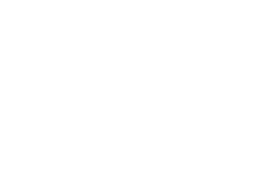
\includegraphics[width=0.5\textwidth]{./img/projection_inv}
            \caption{Projection of $\mathbf{x}$ onto $\mathbf{y}$.}
            \label{fig:projection-png}
        \end{figure}

    \item \textbf{Cauchy space}\\

        A sequence of points in a metric space $x_0, x_1, x_2, \ldots$ is a
        \textit{Cauchy sequence} if it converges, i.e., for any
        $\epsilon > 0$, there exists an integer  $N > 0$ so that the following
        is true for any $m,n > N$:

        \begin{equation}
            d(x_{m}, x_{n}) < \epsilon
        .\end{equation}

        If the limit of any Cauchy sequence of points in the space is also in the
        space, the space is called \textit{complete}, referred to as a
        \textit{Cauchy space}.

\end{itemize}


\chapter{Orthogonal Basis and Gram-Schmidt Process}

From \url{http://fourier.eng.hmc.edu/e176/lectures/algebra/node2.html}\\

Assume \textit{n}-D vector space $\mathbb{R}^{n}$ or $\mathbb{C}^{n}$ is spanned
by a set of \textit{n} independent basis vectors $\begin{bmatrix} \mathbf{v}_1 & \ldots & \mathbf{v}_n \end{bmatrix}$,
not necessarily orthogonal, so that any vector $\mathbf{x} \in \mathbb{R}^{n}$
can be represented as a linear combination of the basis vectors:

\begin{equation}
    \mathbf{x}
    = \sum_{i=1}^{n} c_{i} \mathbf{v}_{i}
    = \begin{bmatrix} \mathbf{v}_1 & \ldots & \mathbf{v}_n \end{bmatrix}
    \begin{bmatrix} c_1\\ \vdots\\ c_n \end{bmatrix}
    = \mathbf{V} \mathbf{c}
,\end{equation}

where $\mathbf{V} = \begin{bmatrix} \mathbf{v}_1 & \ldots & \mathbf{v}_n \end{bmatrix}$ is an
$m \times n$ matrix composed of the $n$ vectors and the coefficients in
$\mathbf{c} = \begin{bmatrix} c_1 & \ldots & c_n \end{bmatrix}^{T}$ can be
found by solving the lienar equation system to get
$\mathbf{c} = \mathbf{V}^{-1}\mathbf{x}$ with complexity $\mathit{O}(n^{3})$.\\

These linearly independent vectors $\mathbf{v}_{1}, \ldots, \mathbf{v}_{n}$ can be
converted into a set of orthogonal vectors $\begin{Bmatrix} \mathbf{u}_1 & \ldots & \mathbf{u}_n \end{Bmatrix}$
satisfying $\mathbf{u}_{i}^{T}\mathbf{u}_{j} = 0 (i \neq j)$ by the following
\textit{Gram-Schmidt process}:

\begin{equation}
    \begin{array}{l}
        \mathbf{u}_{1} = \mathbf{v}_{1}\\
        \mathbf{u}_{2} = \mathbf{v}_{2} - \mathbf{p}_{\mathbf{u}_{1}}(\mathbf{v}_{2})
        = \mathbf{v}_{2} - \left( \frac{\mathbf{v}_{2}^{T}\mathbf{u}_{1}}{\mathbf{u}_{1}^{T}\mathbf{u}_{1}} \right) \mathbf{u}_{1}\\
        \mathbf{u}_{3} = \mathbf{v}_{3}
        - \mathbf{p}_{\mathbf{u}_{1}}(\mathbf{v}_{3})
        - \mathbf{p}_{\mathbf{u}_{2}}(\mathbf{v}_{3})
        = \mathbf{v}_{3}
        - \left( \frac{\mathbf{v}_{3}^{T}\mathbf{u}_{1}}{\mathbf{u}_{1}^{T}\mathbf{u}_{1}} \right) \mathbf{u}_{1}
        - \left( \frac{\mathbf{v}_{3}^{T}\mathbf{u}_{2}}{\mathbf{u}_{2}^{T}\mathbf{u}_{2}} \right) \mathbf{u}_{2}\\
        \ldots \ldots \ldots\\
        \mathbf{u}_{k}
        = \mathbf{v}_{k}
        - \sum_{i=1}^{k-1} \mathbf{p}_{\mathbf{u}_{i}}(\mathbf{v}_{k})
        = \mathbf{v}_{k}
        - \sum_{i=1}^{k-1} \left( \frac{\mathbf{v}_{k}^{T}\mathbf{u}_{i}}{\mathbf{u}_{i}^{T}\mathbf{u}_{i}} \right) \mathbf{u}_{i}.
    \end{array}
\end{equation}

where $\mathbf{p}_{\mathbf{u}_{i}}(\mathbf{v}_{k})$ is the projection of
$\mathbf{v}_{k}$ onto $\mathbf{u}_{i}$:

\begin{equation}
    \mathbf{p}_{\mathbf{u}_{i}}(\mathbf{v}_{k})
    = \left( \frac{\mathbf{v}_{k}^{T}\mathbf{u}_{i}}{\mathbf{u}_{i}^{T}\mathbf{u}_{i}} \right) \mathbf{u}_{i}
.\end{equation}

We see that $\mathbf{u}_{2}$ so obtained is indeed orthogonal to all
$\mathbf{u}_{1}$:

\begin{equation}
    \mathbf{u}_{2}^{T}\mathbf{u}_{1}
    = \left[ \mathbf{v}_{2}
        - \left( \frac{\mathbf{v}_{2}^{T}\mathbf{u}_{1}}
        {\mathbf{u}_{i}^{T}\mathbf{u}_{1}} \right)
        \mathbf{u}_{i} \right]^{T} \mathbf{u}_{1}
    = \mathbf{v}_{2}^{T}\mathbf{u}_{1}
    - \frac{\mathbf{v}_{2}^{T}\mathbf{u}_{1}}{\mathbf{u}_{1}^{T}\mathbf{u}_{1}}
    \mathbf{u}_{1}^{T}\mathbf{u}_{1} = 0
,\end{equation}

and, by mathematical induction, we can further prove that $\mathbf{u}_{k}^{T}\mathbf{u}_{i} = 0$
for all $i = 1, \ldots, k-1$. In other words, $\mathbf{u}_{k}$ is the component
of $\mathbf{v}_{k}$ that is orthogonal to all previously found orthogonal vectors
$\mathbf{u}_{1}, \ldots, \mathbf{u}_{k-1}$.

\begin{figure}[h]
    \centering
    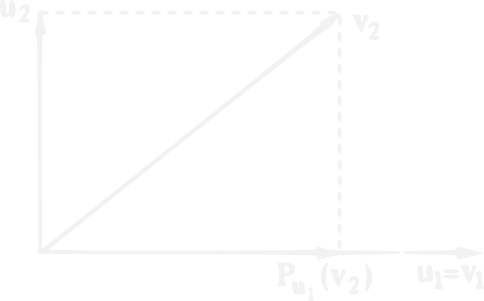
\includegraphics[width=0.7\textwidth]{./img/GramSchmidt_inv}
    \caption{$\mathbf{u}_{2} = \mathbf{v}_{2} - \mathbf{p}_{\mathbf{u}_{1}}(\mathbf{v}_{2})$}
    \label{fig:GramSchmidt}
\end{figure}

Given a set of orthogonal basis $\begin{Bmatrix} \mathbf{u}_1 & \ldots & \mathbf{u}_n \end{Bmatrix}$
satisfying $\langle \mathbf{u}_{i}, \mathbf{u}_{j} \rangle = \mathbf{u}_{i}^{T}\mathbf{u}_{j} = 0$
for any $\mathbf{i \neq j}$, we can again represent any given vector $\mathbf{x}$
as a linear combination of these bases as:

\begin{equation}
    \mathbf{x} = \sum_{i=1}^{n} d_{i} \mathbf{u}_{i}
.\end{equation}

The coefficients $d_{i}$ can now be obtained easily. Premultiplying
$\mathbf{u}_{j}^{T}$ on both sides of the equation above, we get:

\begin{equation}
    \mathbf{u}_{j}^{T} \mathbf{x}
    = \mathbf{u}_{j}^{T} \left(
    \sum_{i=1}^{n} d_{i} \mathbf{u}_{i}\right)
    = \sum_{i=1}^{n} d_{i} \mathbf{u}_{j}^{T} \mathbf{u}_{i}
    = d_{j} \mathbf{u}_{j}^{T} \mathbf{u}_{j}
.\end{equation}

\begin{bbox}[1.0]
\textit{Note:}
    $\sum_{i=1}^{n} d_{i} \mathbf{u}_{j}^{T} \mathbf{u}_{i} = d_{j} \mathbf{u}_{j}^{T} \mathbf{u}_{j}$
    because $\mathbf{u}_{i}^{T} \mathbf{u}_{j} \neq 0 \iff i = j$ \textit{(Tomek)}
\end{bbox}

Solving for $d_{j}$ we get:

\begin{equation}
    d_{j} = \frac{\mathbf{u}_{j}^{T}\mathbf{x}}{\mathbf{u}_{j}^{T}\mathbf{u}_{j}},
    \qquad j = 1, \ldots, n
.\end{equation}

As the $n$ coefficients are decoupled, each of them can be obtained separately
with linear computational complexity $O(n)$ with total complexity  $I(n^{2}$
for all $n$ of them. The complexity is reduced to $O(n^{2})$ from $O(n^{3})$
for solving the equation system $mathbf{c} = mathbf{V}^{-1}mathbf{b}$, needed in the case
where the basis is not orthogonal. This is the reason why orthogonal bases are
preferred in general. Now the vector $mathbf{x}$ can be written as:

\begin{equation}
    \mathbf{x} = \sum_{i=1}^{n} d_{i} \mathbf{u}_{i}
    = \sum_{i=1}^{n} \left(
    \frac{\mathbf{u}_{j}^{T}\mathbf{x}}{\mathbf{u}_{j}^{T}\mathbf{u}_{j}}
    \right) \mathbf{u}_{i}
    = \sum_{i=1}^{n} \mathbf{p}_{\mathbf{u}_{i}}(\mathbf{x})
,\end{equation}

where the ith term of the summation above is simply the projection
$\mathbf{p}_{\mathbf{u}_{i}}(\mathbf{x})$ of $\mathbf{x}$ onto the ith basis of $\mathbf{u}_{i}$.\\

The concept of orthogonal vectors satisfying $\mathbf{u}^{T}\mathbf{v} = 0$
can be generalised to \textit{conjugate vectors} that satisfy
$\mathbf{u}^{T}\mathbf{A}\mathbf{v} = 0$ with respect to a symmetric matrix
$\mathbf{A} = \mathbf{A}^{T}$. This can be expressed in the form of inner product:

\begin{equation}
    \mathbf{u}^{T} \mathbf{A} \mathbf{v}
    = (\mathbf{A}\mathbf{v})^{T}\mathbf{u}
    = \mathbf{v}^{T}\mathbf{A}\mathbf{u}
.\end{equation}

Conjugate vectors with respect to $\mathbf{A}$ can also be considered as orthogonal
to each other with respect to $\mathbf{A}$. Two orthogonal vectors satisfying
$\mathbf{u}^{T}\mathbf{v} = 0$ can be considered as a special case of conjugate
vectors with respect to $\mathbf{A} = \mathbf{I}$.\\

Based on this generalized orthogonality, we can also define the projection of
$\mathbf{v}$ onto $\mathbf{u}$ with respect to $\mathbf{A}$ as:

\begin{equation}
    \mathbf{p}_{\mathbf{u}}(\mathbf{v}) = \left(
    \frac{\mathbf{u}^{T}\mathbf{A}\mathbf{v}}{\mathbf{u}^{T}\mathbf{A}\mathbf{u}}
    \right) \mathbf{u}
.\end{equation}

Given a set of A-conjugate basis vectors $\begin{Bmatrix} d_1 & \ldots & d_n \end{Bmatrix}$
satisfying $\mathbf{d}_{i}^{T}\mathbf{A}\mathbf{d}_{j} = 0$ for any $\mathbf{i \neq j}$,
we can represent any $\mathbf{x}$ as:

\begin{equation}
    \mathbf{x} = \sum_{i=1}^{n} a_{i}\mathbf{d}_{i}
.\end{equation}

The coefficients $a_{i}$ can be obtained by pre-multiplying $\mathbf{d}_{j}^{T}\mathbf{A}$
on both sides:

\begin{equation}
    \mathbf{d}_{j}^{T}\mathbf{A}\mathbf{x}
    = \sum_{i=1}^{n} a_{i}\mathbf{d}_{j}^{T}\mathbf{A}\mathbf{d}_{i}
    = a_{j}\mathbf{d}_{j}^{T}\mathbf{A}\mathbf{d}_{j}
.\end{equation}

Solving for $a_{i}$ we get:

\begin{equation}
    a_{j} = \frac{\mathbf{d}_{j}^{T}\mathbf{A}\mathbf{x}}{\mathbf{d}_{j}^{T}\mathbf{A}\mathbf{d}_{j}}
    ,\qquad j = 1,\ldots,n
.\end{equation}

and $\mathbf{x}$ is now represented as the sum of its A-projections onto the
\textit{n} basis vectors $\begin{Bmatrix} d_1 & \ldots & d_n \end{Bmatrix}$:

\begin{equation}
    \mathbf{x}
    = \sum_{i=1}^{n} a_{i}\mathbf{d}_{i}
    = \sum_{i=1}^{n} \left(
    \frac{\mathbf{s}_{i}^{T}\mathbf{A}\mathbf{x}}{\mathbf{d}_{i}^{T}\mathbf{A}\mathbf{d}_{i}}
    \right) \mathbf{d}_{i}
    = \sum_{i=1}^{n} \mathbf{p}_{\mathbf{d}_{i}}(\mathbf{x})
.\end{equation}

A set of independent basis vectors $\begin{Bmatrix} v_1 & \ldots & v_n \end{Bmatrix}$
can now be also converted to an orthogonal basis with respect to a symmetric
vector $\mathbf{A}$ by a Gram-Schmidt process:

\begin{equation}
    \mathbf{d}_{k} = \mathbf{v}_{k}
    - \sum_{i=1}^{k-1} \mathbf{p}_{\mathbf{d}_{i}}(\mathbf{v}_{k})
    = \mathbf{v}_{k}
    - \sum_{i=1}^{k-1} \left(
    \frac{\mathbf{v}_{k}^{T}\mathbf{A}\mathbf{d}_{i}}
    {\mathbf{d}_{i}^{T}\mathbf{A}\mathbf{d}_{i}} \right) \mathbf{d}_{i}
    , \qquad (k = 1, \ldots, n)
.\end{equation}


\chapter{Properties of Matrices}
Rank, Trace, Determinant, Transpose and Inverse of Matrices\\

From: \url{http://fourier.eng.hmc.edu/e176/lectures/algebra/node3.html}\\

Let $\mathbf{A}$ be an $m \times n$ square matrix:

\begin{equation}
    \mathbf{A} = \begin{bmatrix} a_1 & \ldots & a_n \end{bmatrix}
    = \begin{bmatrix}
        a_{11} & \ldots & a_{1n}\\
        \vdots & \ddots & \vdots\\
        a_{m1} & \ldots & a_{mn}
    \end{bmatrix}_{m \times n}
\end{equation}

where:

\begin{equation}
    \mathbf{a}_{j} = \begin{bmatrix} a_{1j}\\ \vdots\\ a_{mj} \end{bmatrix}
    ,\qquad (j = 1, \ldots, n)
\end{equation}

is the $j^{th}$ column vector and

\begin{equation}
    \begin{bmatrix} a_{i1} & \ldots & a_{in} \end{bmatrix}
    , \qquad (i = 1, \ldots, m)
\end{equation}

is the $i^{th}$ row vector. If $m = n$, $\mathbf{A}$ is a \textit{square matrix}.
In particular, if all entries of a square matrix are zero except those along the
diagonal, it is a \textit{diagonal matrix}. Morover, if the diagonal entries of
a diagonal matrix are all one, it is the \textit{identity matrix}:

\begin{equation}
    \mathbf{I} = \begin{bmatrix}
        1 & 0 & \ldots & 0\\
        0 & 1 &   & \vdots\\
        \vdots & & \ddots & 0\\
        0 & \ldots & 0 & 1
    \end{bmatrix}
.\end{equation}

\begin{itemize}
    \item \textbf{Rank}\\

        The $m$ row vectors span the \textit{row space} of $\mathbf{A}$ and the
        $n$ columns span the \textit{column space} of $\mathbf{A}$. The \textit{rank}
        of each space is its dimension, the number of independent vectors in the
        space. The row and column spaces have the same rank, which is also the
        rank of matrix $\mathbf{A}$, i.e.:

        \begin{equation}
            r = rank(\mathbf{A}) \le \min(m, n)
        .\end{equation}

        In other words, the rank of matrix $\mathbf{A}$ is the number of its
        independent rows or columns.

     \item \textbf{Transpose}\\

        The \textit{transpose} $\mathbf{x}^{T}$ of a column vector $\mathbf{x}$
        is a row vector:

        \begin{equation}
            \mathbf{x}^{T} = \begin{bmatrix} x_1\\ \vdots\\ x_n \end{bmatrix}^{T}
            = \begin{bmatrix} x_1 & \ldots & x_n \end{bmatrix}
        .\end{equation}

        The transpose $\mathbf{A}^{T}$ of a matrix $\mathbf{A}$ is obtained
        by switching the position of elements $a_{ij}$ and $a_{ji}$,
        for all $i \in \{1, \ldots, m\}$ and $j \in \{1, \ldots, n\}$.
        In other words, the $i^{th}$ column of $\mathbf{A}$ becomes the
        $i^{th}$ row of $\mathbf{A}^{T}$.\\

        The properties of the transpose:

        \begin{itemize}
            \item $(\mathbf{A}^{T})^{T} = \mathbf{A}$,

            \item $(\mathbf{A} + \mathbf{B})^{T} = \mathbf{A}^{T} + \mathbf{B}^{T}$,

            \item $(\mathbf{A}\mathbf{B})^{T} = \mathbf{B}^{T}\mathbf{A^{T}}$,

            \item $\mathbf{A}^{T}$ and $\mathbf{A}$ have the same eigenvalues
                and eigenvectors.
        \end{itemize}

        If $\mathbf{A} = \mathbf{A}^{T}$, it is a \textit{symmetric matrix}.

    \item \textbf{Conjugate transpose}\\

        The \textit{conjugate transpose} of a matrix $\mathbf{A}$, denoted by
        $\mathbf{A}^{*}$, is by taking the complex conjugate of its transpose:

        \begin{equation}
            \mathbf{A}^{*} = (\overline{\mathbf{A}})^{T} = \overline{\mathbf{A}^{T}}
        ,\end{equation}

        i.e., $(\mathbf{A}^{*})_{ij} = \overline{\mathbf{A}}_{ji}$, the $ij^{th}$
        entry of $\mathbf{A}^{*}$ is the complex conjugate of the $ji^{th}$ entry
        of $\mathbf{A}$.

        The properties of the conjugate transpose:

        \begin{itemize}
            \item $(\mathbf{A}^{*})^{*} = \mathbf{A}$
            \item $(c \mathbf{A})^{*} = \overline{c}\mathbf{A}^{*}$
            \item $(\mathbf{A} + \mathbf{B})^{*} = \mathbf{A}^{*} + \mathbf{B}^{*}$
            \item $(\mathbf{A}\mathbf{B})^{*} = \mathbf{B}^{*}\mathbf{A}^{*}$
            \item $\det(\mathbf{A}^{*}) = (\det \mathbf{A})^{*} = \overline{\det \mathbf{A}}$
            \item $tr(\mathbf{A}^{*}) = (tr \mathbf{A})^{*} = \overline{tr \mathbf{A}}$
            \item $(\mathbf{A^{*}})^{-1} = (\mathbf{A}^{-1})^{*}$
            \item The eigenvalues of $\mathbf{A}^{*}$ are the complex conjugates
                of the eigenvalues of $\mathbf{A}$. (But their eigenvectors are
                not related.)
            \item $\langle \mathbf{A}\mathbf{x}, \mathbf{y} \rangle = \langle \mathbf{x}, \mathbf{A}^{*}\mathbf{y} \rangle$
        \end{itemize}

        \textbf{Proof:}

        \begin{equation}
            \langle \mathbf{A}\mathbf{x}, \mathbf{y} \rangle
            = (\mathbf{A}\mathbf{x})^{*}\mathbf{y}
            = \mathbf{x}^{*}\mathbf{A}^{*}\mathbf{y}
            = \mathbf{x}^{*}(\mathbf{A}^{*}\mathbf{y})
            = \langle \mathbf{x}, \mathbf{A}^{*}\mathbf{y} \rangle
        .\end{equation}

        If $\mathbf{A} = \mathbf{A}^{*}$, it is a \textit{Hermitian matrix}.
        A real Hermitian matrix is a symmetric matrix. The inverse of an invertible
        Hermitian matrix is also Hermitian, i.e., if $\mathbf{A} = \mathbf{A}^{*}$,
        then $(\mathbf{A}^{-1})^{*} = \mathbf{A}^{-1}$.

    \item \textbf{Trace}\\

        The \textit{trace} of a square matrix $A$ is the sum of its diagonal elements:

        \begin{equation}
            tr(\mathbf{A}) = \sum_{i=1}^{n} a_{ii}
        .\end{equation}

        The properties of the trace:

        \begin{itemize}
            \item $tr(c \mathbf{A}) = c \; tr(\mathbf{A})$
            \item $tr(\mathbf{A}^{T}) = tr(\mathbf{A})$
            \item $tr(\mathbf{A} + \mathbf{B}) = tr(\mathbf{B} + \mathbf{A})$
            \item $tr(\mathbf{A} \mathbf{B}) = tr(\mathbf{B} \mathbf{A})$
            \item $tr(\mathbf{A}^{T} \mathbf{B}) = tr(\mathbf{A} \mathbf{B}^{T})$
            \item $tr(\mathbf{R}^{-1} \mathbf{A} \mathbf{R})
                = tr(\mathbf{R}^{-1}(\mathbf{A} \mathbf{R}))
                = tr((\mathbf{A} \mathbf{R}) \mathbf{R}^{-1})
                = tr(\mathbf{A})$
        \end{itemize}

    \item \textbf{Determinant}\\

        The \textit{determinant} of a square matrix $\mathbf{A}$ is denoted by
        $\det(\mathbf{A}) = |\mathbf{A}|$, and $\det(\mathbf{A}) \neq 0$ if and
        only if it is full rank, i.e., $rank(\mathbf{A}) = n$.\\

        The properties of the determinant:

        \begin{itemize}
            \item $\det(\mathbf{I}) = 1$,
            \item $\det(\mathbf{A}^{T}) = \det(\mathbf{A})$,
            \item $\det(\mathbf{A}^{-1}) = \det(\mathbf{A})^{-1}$,
            \item $\det(\mathbf{A}\mathbf{B}) = \det(\mathbf{A})\det(\mathbf{B})$,
            \item $\det(c\mathbf{A}) = c^{n} \det(\mathbf{A})$.
        \end{itemize}

    \item \textbf{Inverse}\\

        If $\mathbf{A}$ is an $m \times n$ full rank square matrix with $m = n = r$,
        then there exists an  \textit{inverse matrix} $\mathbf{A}^{-1}$ that
        satisfies $\mathbf{A}\mathbf{A}^{-1} = \mathbf{A}^{-1}\mathbf{A} = \mathbf{I}$.
        The inverse $\mathbf{A}^{-1}$ does not exist if $\mathbf{A}$ is not
        square $(m \neq n)$ or full rank $(r < m = n)$.\\

        The properties of the inverse:

        \begin{itemize}
            \item $(\mathbf{A}^{-1})^{-1} = \mathbf{A}$,
            \item $(\mathbf{A}^{T})^{-1} = (\mathbf{A}^{-1})^{T}$,
            \item $\det(\mathbf{A}^{-1}) = \det(\mathbf{A})^{-1}$,
            \item $(\mathbf{A}\mathbf{B})^{-1} = \mathbf{B}^{-1}\mathbf{A}^{-1}$.
        \end{itemize}

        For example, the solution of a linear equation system
        $\mathbf{A}\mathbf{x} = \mathbf{b}$ of $m$ equations and $n = m$ variables
        can be obtained as $\mathbf{x} = \mathbf{A}^{-1}\mathbf{b}$.
\end{itemize}






\chapter{Inverse and Determinant of Partitioned Symmetric Matrices}
From \url{http://fourier.eng.hmc.edu/e176/lectures/algebra/node7.html}\\

\begin{itemize}
    \item \textbf{Theorem 1 (Woodbury identity)}

        \begin{equation}
            (\mathbf{A} + \mathbf{C} \mathbf{B} \mathbf{D})^{-1} =
            \mathbf{A}^{-1} - \mathbf{A}^{-1} \mathbf{C} (\mathbf{B}^{-1} + \mathbf{D} \mathbf{A}^{-1} \mathbf{C})^{-1} \mathbf{D} \mathbf{A}^{-1}
        .\end{equation}

        \textbf{Proof:}

        \begin{equation}
            \begin{array}{l}
                (\mathbf{A} + \mathbf{C} \mathbf{B} \mathbf{D}) [\mathbf{A}^{-1} - \mathbf{A}^{-1} \mathbf{C} (\mathbf{B}^{-1} + \mathbf{D} \mathbf{A}^{-1} \mathbf{C})^{-1} \mathbf{D} \mathbf{A}^{-1}]\\
                = (\mathbf{A} + \mathbf{C} \mathbf{B} \mathbf{D}) \mathbf{A}^{-1} - (\mathbf{A} + \mathbf{C} \mathbf{B} \mathbf{D}) \mathbf{A}^{-1} \mathbf{C} ( \mathbf{B}^{-1} + \mathbf{D} \mathbf{A}^{-1} \mathbf{C})^{-1} \mathbf{D} \mathbf{A}^{-1}\\
                = \mathbf{I} + \mathbf{C} \mathbf{B} \mathbf{D} \mathbf{A}^{-1} - (\mathbf{C} + \mathbf{C} \mathbf{B} \mathbf{D} \mathbf{A}^{-1} \mathbf{C}) (\mathbf{B}^{-1} + \mathbf{D} \mathbf{A}^{-1} \mathbf{C})^{-1} \mathbf{D} \mathbf{A}^{-1}\\
                = \mathbf{I} + \mathbf{C} \mathbf{B} \mathbf{D} \mathbf{A}^{-1} - \mathbf{C} \mathbf{B} (\mathbf{B}^{-1} + \mathbf{D} \mathbf{A}^{-1} \mathbf{C}) (\mathbf{B}^{-1} + \mathbf{D} \mathbf{A}^{-1} \mathbf{C})^{-1} \mathbf{D} \mathbf{A}^{-1}\\
                = \mathbf{I} + \mathbf{C} \mathbf{B} \mathbf{D} \mathbf{A}^{-1} - \mathbf{C} \mathbf{B} \mathbf{D} \mathbf{A}^{-1} = \mathbf{I}.
            \end{array}
        \end{equation}

        In particular, if $\mathbf{C} = \mathbf{D} = \mathbf{I}$, then we have

        \begin{equation}
            (\mathbf{A} + \mathbf{B})^{-1} = \mathbf{A}^{-1} - \mathbf{A}^{-1} (\mathbf{A}^{-1} + \mathbf{B}^{-1})^{-1} \mathbf{A}^{-1}
        .\end{equation}

    \item \textbf{Theorem 2} (inverse of a partitioned symmetric matrix)\\

        Divide an $n \times n$ symmetric matrix $\mathbf{A}$ into four blocks:

        \begin{equation}
            \mathbf{A} = \begin{bmatrix}
                \mathbf{A}_{11} & \mathbf{A}_{12}\\
                \mathbf{A}_{21} & \mathbf{A}_{22}
            \end{bmatrix}
        .\end{equation}

        The inverse matrix $\mathbf{B} = \mathbf{A}^{-1}$ can also be divided into four blocks:

        \begin{equation}
            \mathbf{B} = \mathbf{A}^{-1} = \begin{bmatrix}
                \mathbf{B}_{11} & \mathbf{B}_{12}\\
                \mathbf{B}_{21} & \mathbf{B}_{22}
            \end{bmatrix}
        .\end{equation}

        Here we assume the dimensionalities of these blocks are:
        \begin{itemize}
            \item $\mathbf{A}_{11}$ and $\mathbf{B}_{11}$ are $p \times p$,
            \item $\mathbf{A}_{22}$ and $\mathbf{B}_{22}$ are $q \times q$,
            \item $\mathbf{A}_{12} = \mathbf{A}_{21}^{T}$ and $\mathbf{B}_{12} = \mathbf{B}_{21}^{T}$ are $p \times q$,
        \end{itemize}
        with $p + q = n$. Then we have

         \begin{equation}
            \begin{array}{ll}
                \mathbf{B}_{11} &= (\mathbf{A}_{11} - \mathbf{A}_{12} \mathbf{A}_{22}^{-1} \mathbf{A}_{21})^{-1}\\
                       &= \mathbf{A}_{11}^{-1} + \mathbf{A}_{11}^{-1} \mathbf{A}_{12} (\mathbf{A}_{22} - \mathbf{A}_{21} \mathbf{A}_{11}^{-1} \mathbf{A}_{12})^{-1} \mathbf{A}_{21} \mathbf{A}_{11}^{-1}\\

                \mathbf{B}_{22} &= (\mathbf{A}_{22} - \mathbf{A}_{21} \mathbf{A}_{11}^{-1} \mathbf{A}_{12})\\
                       &= \mathbf{A}_{22}^{-1} + \mathbf{A}_{22}^{-1} \mathbf{A}_{21} (\mathbf{A}_{11} - \mathbf{A}_{12} \mathbf{A}_{22}^{-1} \mathbf{A}_{21})^{-1} \mathbf{A}_{12} \mathbf{A}_{22}^{-1}\\

                \mathbf{B}_{21} &= - \mathbf{A}_{22}^{-1} \mathbf{A}_{21} (\mathbf{A}_{11} - \mathbf{A}_{12} \mathbf{A}_{22}^{-1} \mathbf{A}_{21})^{-1}\\
                \mathbf{B}_{12} &= - \mathbf{A}_{11}^{-1} \mathbf{A}_{12} (\mathbf{A}_{22} - \mathbf{A}_{21} \mathbf{A}_{11}^{-1} \mathbf{A}_{12})^{-1}
            \end{array}
        \end{equation}

        \textbf{Proof:}

        \begin{equation}
            \begin{array}{ll}
                \mathbf{I}_{n} &= \mathbf{A} \mathbf{A}^{-1} = \mathbf{A} \mathbf{B} =
                \begin{bmatrix}
                    \mathbf{A}_{11} & \mathbf{A}_{12}\\
                    \mathbf{A}_{21} & \mathbf{A}_{22}
                \end{bmatrix}
                \begin{bmatrix}
                    \mathbf{B}_{11} & \mathbf{B}_{12}\\
                    \mathbf{B}_{21} & \mathbf{B}_{22}
                \end{bmatrix}\\
                               &=
                \begin{bmatrix}
                    \mathbf{A}_{11} \mathbf{B}_{11} + \mathbf{A}_{12} \mathbf{B}_{12} & \mathbf{A}_{11} \mathbf{B}_{12} + \mathbf{A}_{12} \mathbf{B}_{22}\\
                    \mathbf{A}_{21} \mathbf{B}_{11} + \mathbf{A}_{22} \mathbf{B}_{21} & \mathbf{A}_{21} \mathbf{B}_{12} + \mathbf{A}_{22} \mathbf{B}_{22}
                \end{bmatrix} =
                \begin{bmatrix}
                    \mathbf{I}_{p} & \mathbf{0}\\
                    \mathbf{0} & \mathbf{I}_{q}
                \end{bmatrix}
            \end{array}
        \end{equation}

        Equate each of the four blocks to get:

        \begin{equation}
            \begin{array}{lcl}
                \mathbf{A}_{11} \mathbf{B}_{11} + \mathbf{A}_{12} \mathbf{B}_{12} = \mathbf{I}_{p}, & \text{ or } & \mathbf{B}_{11} = \mathbf{A}_{11}^{-1} - \mathbf{A}_{11}^{-1} \mathbf{A}_{12} \mathbf{B}_{21} \\
                \mathbf{A}_{11} \mathbf{B}_{12} + \mathbf{A}_{12} \mathbf{B}_{22} = \mathbf{0}, & \text{ or } & \mathbf{B}_{12} = - \mathbf{A}_{11}^{-1} \mathbf{A}_{12} \mathbf{B}_{22} \\
                \mathbf{A}_{21} \mathbf{B}_{11} + \mathbf{A}_{22} \mathbf{B}_{21} = \mathbf{0}, & \text{ or } & \mathbf{B}_{21} - \mathbf{A}_{22}^{-1} \mathbf{A}_{21} \mathbf{B}_{11} \\
                \mathbf{A}_{21} \mathbf{B}_{12} + \mathbf{A}_{22} \mathbf{B}_{22} = \mathbf{I}_{q}, & \text{ or } & \mathbf{B}_{22} = \mathbf{A}_{22}^{-1} - \mathbf{A}_{22}^{-1} \mathbf{A}_{21} \mathbf{B}_{12}
            \end{array}
        \end{equation}

        Plug $\mathbf{B}_{21}$ into $\mathbf{B}_{11}$ to get:

        \begin{equation}
            \mathbf{B}_{11} = \mathbf{A}_{11}^{-1} + \mathbf{A}_{11}^{-1} \mathbf{A}_{12} \mathbf{A}_{22}^{-1} \mathbf{A}_{21} \mathbf{B}_{11}
        .\end{equation}

        Solve for $\mathbf{B}_{11}$ to get:

        \begin{equation}
            \mathbf{B}_{11} = (\mathbf{A}_{11} - \mathbf{A}_{12} \mathbf{A}_{22}^{-1} \mathbf{A}_{21})^{-1}
        .\end{equation}

        Applying theorem 1 to this expression, we also get the other expression in the theorem.
        Similarily we can get:

        \begin{equation}
            \begin{array}{ll}
                \mathbf{B}_{22} = (\mathbf{A}_{22} - \mathbf{A}_{21} \mathbf{A}_{11}^{-1} \mathbf{A}_{12})^{-1} \\
                \mathbf{B}_{21} = - \mathbf{A}_{22}^{-1} \mathbf{A}_{21} (\mathbf{A}_{11} - \mathbf{A}_{12} \mathbf{A}_{22}^{-1} \mathbf{A}_{21})^{-1} \\
                \mathbf{B}_{12} = - \mathbf{A}_{11}^{-1} \mathbf{A}_{12} (\mathbf{A}_{22} - \mathbf{A}_{21} \mathbf{A}_{11}^{-1} \mathbf{A}_{12}^{-1})^{-1}
            \end{array}
        \end{equation}

    \item \textbf{Theorem 3} (Determinant of a partitioned symmetric matrix)

        \begin{equation}
            \begin{array}{ll}
                |\mathbf{A}|  &= \left|
                \begin{bmatrix}
                    \mathbf{A}_{11} & \mathbf{A}_{12}\\
                    \mathbf{A}_{21} \mathbf{A}_{22}
                \end{bmatrix}  \right|\\
                              &=
                |\mathbf{A}_{22}| |\mathbf{A}_{11} - \mathbf{A}_{12} \mathbf{A}_{22}^{-1} \mathbf{A}_{21}|
                = |\mathbf{A}_{11}| |\mathbf{A}_{22} - \mathbf{A}_{21} \mathbf{A}_{11}^{-1} \mathbf{A}_{12}|
            \end{array}
        \end{equation}

        \textbf{Proof:}

        \begin{equation}
            \begin{array}{ll}
                A = \begin{bmatrix}
                    \mathbf{A}_{11} & \mathbf{A}_{12}\\
                    \mathbf{A}_{21} 7 \mathbf{A}_{22}
                \end{bmatrix} &= \begin{bmatrix}
                    \mathbf{A}_{11} & \mathbf{0}\\
                    \mathbf{A}_{21} & \mathbf{I}
                \end{bmatrix} \begin{bmatrix}
                    \mathbf{I} & \mathbf{A}_{11}^{-1} \mathbf{A}_{12}\\
                    0 & \mathbf{A}_{22} - \mathbf{A}_{21} \mathbf{A}_{11}^{-1} \mathbf{A}_{12}
                \end{bmatrix}\\
                &= \begin{bmatrix}
                    \mathbf{I} & \mathbf{A}_{12}\\
                    \mathbf{0} & \mathbf{A}_{22}
                \end{bmatrix} \begin{bmatrix}
                    \mathbf{A}_{11} - \mathbf{A}_{12} \mathbf{A}_{22}^{-1} \mathbf{A}_{21} & \mathbf{0}\\
                    \mathbf{A}_{22}^{-1} \mathbf{A}_{21} & \mathbf{0}
                \end{bmatrix}
            \end{array}
        \end{equation}

        The theorem is proved as we also know that

        \begin{equation}
            |\mathbf{B} \mathbf{C}| = |\mathbf{B}| |\mathbf{C}|
        \end{equation}

        and

        \begin{equation}
            \begin{vmatrix}
                \mathbf{B} & \mathbf{0}\\
                \mathbf{X} & \mathbf{C}
            \end{vmatrix} = \begin{vmatrix}
                \mathbf{B} & \mathbf{X}\\
                \mathbf{0} & \mathbf{C}
            \end{vmatrix} = |\mathbf{B}| |\mathbf{C}|
        .\end{equation}
\end{itemize}




\chapter{Unitary Transform}
From \url{http://fourier.eng.hmc.edu/e176/lectures/algebra/node8.html}\\

Given any \textit{unitary matrix} $\mathbf{A}$ satisfying $\mathbf{A} \mathbf{A}^{*} = \mathbf{A}^{*} \mathbf{A} = \mathbf{I}$, we can define a \textit{unitary transform} of a vector $\mathbf{x} = [x_{1}, \dots, x_{n}]^{T}$:
\begin{equation}
\left\{
    \begin{array}{lr}
        \mathbf{y}
        = \begin{bmatrix}
            \mathbf{y}_{1}\\
            \dots\\
            \mathbf{y}_{n}
        \end{bmatrix}
        = \mathbf{A}^{*} \mathbf{x}
        = \begin{bmatrix}
             \bar{a}_{1}^{T} \\
             \vdots  \\
             \bar{a}_{n}^{T}
        \end{bmatrix}
        \begin{bmatrix}
            x_{1}\\
            \vdots \\
            x_{n}
        \end{bmatrix}, & \text{(forward transform)}\\

        \mathbf{x}
        = \begin{bmatrix}
            \mathbf{x}_{1}\\
            \dots\\
            \mathbf{x}_{n}
        \end{bmatrix}
        = \mathbf{A} \mathbf{y}
        = \begin{bmatrix}
            a_{1} & \dots & a_{n}
        \end{bmatrix}
        \begin{bmatrix}
            y_{1}\\
            \vdots\\
            y_{n}
        \end{bmatrix}
        = \sum_{i=1}^{n} y_{i} a_{i}. & \text{(inverse transform)}
\end{array}
\right.
\end{equation}

When $\mathbf{A} = \overline{\mathbf{A}}$ is real, $\mathbf{A}^{-1} = \mathbf{A}^{T}$ is an orthogonal matrix and the corresponding transform is an orthogonal transform.\\

The first equation above is the \textit{forward transform} and can be written in component form as:
\begin{equation}
    \begin{array}{lr}
        y_{i} = \overline{\mathbf{a}}_{i}^{T} \mathbf{x}
        = \langle \mathbf{x}, \mathbf{a}_{i} \rangle
        = \sum_{j=1}^{n} x_{j} \overline{a}_{ij}, & (i = 1, \dots, n)
    \end{array}
.\end{equation}

The transform coefficient is an inner product $y_i = \langle \mathbf{x}, \mathbf{a}_i \rangle$, representing the projection of vector $\mathbf{x}$ onto the ith column vector  $\mathbf{a}_i$ of the transform matrix $\mathbf{A}$. The second equation is the \textit{inverse transform} and can also be written in component form as:

\begin{equation}
    \begin{array}{lr}
        x_j = \sum_{i=1}^{n} a_{ji} y_{i}, & (j = 1, \dots, n)
    \end{array}
.\end{equation}

By this transform, vector $\mathbf{x}$ is represented as a linear combination (weighted sum) of the $n$ column vectors  $\mathbf{a}_1, \mathbf{a}_2, \dots, \mathbf{a}_n$ of matrix $\mathbf{A}$. Geometrically,  $\mathbf{x}$ is a point in the n-dimensional space spanned by these $n$ orthonormal basis vectors. Each coefficient (coordinate)  $y_i$ is the projection of  $\mathbf{x}$ onto the corresponding basis vector $\mathbf{a}_i$.

\begin{figure}[htpb]
    \centering
    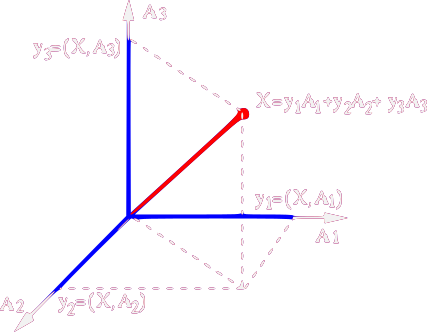
\includegraphics[width=0.7\textwidth]{./img/unitary_transform_1_inv}
    \caption[Unitary transform]{Each coefficient (coordinate) $y_i$ is the projection of ${\bf x}$ onto the corresponding basis vector ${\bf a}_i$}
    \label{fig:unitary_transform_1}
\end{figure}

As the n-dimensional space can be spanned by the column vectors of \textit{any} $n \times n$ unitary (orthogonal) matrix, a vector  $\bf{x}$ in the space can be represented by any of such matrices, each defining a different transform.\\

\textbf{Examples:}
\begin{itemize}
    \item When $\bf{A} = \mathbf{I} = [\dots, \mathbf{e}_i, \dots]$ is an identity matrix, we have
        \begin{equation}
            \mathbf{x} = \sum_{i=1}^{n} y_i \mathbf{a}_i = \sum_{i=1}^{n} x_i \mathbf{e}_i
        \end{equation}

        where $\mathbf{e}_i = [0, \dots, 0, 1, 0, \dots, 0]^{T}$ is the ith column of  $\mathbf{I}$ with the ith element equal 1 and all other 0.

    \item When $a_{mn} = w[m,n] = e^{-j 2 \pi m n / N}$, the corresponding
        transform is discrete Fourrier transform. The nth column vector
        $\mathbf{w}_n$ if the transform matrix
        $\mathbf{W} = [\mathbf{w}_0, \dots, \mathbf{w}_{N-1}]$
        represents a sinusoid of frequency  $n f_0$,
        and the corresponding complex coordinate
        $y_n = (\mathbf{x}, \mathbf{w}_n)$ represents the magnitude
        $|y_n|$ and phase $\angle y_n$
        of this nth frequency component. The Fourrier transform
        $\mathbf{y} = \mathbf{W} \mathbf{x}$ represents a rotation of the coordinate
        system.\\

        \begin{figure}[htpb]
            \centering
            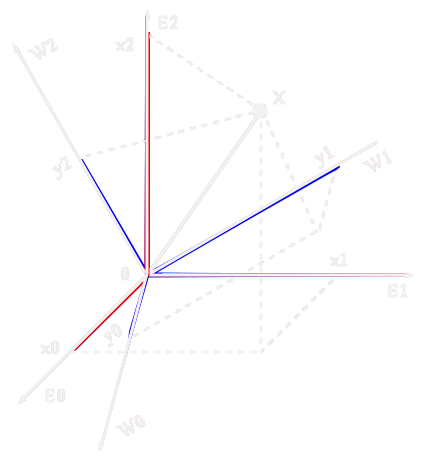
\includegraphics[width=0.7\textwidth]{./img/unitary_transform_2_inv}
            \caption{The Fourrier transform $\mathbf{y} = \mathbf{W} \mathbf{x}$ represents a rotation of the coordinate system.}
            \label{fig:unitary_transform_2}
        \end{figure}

        A unitary (orthogonal if real) transform $\mathbf{y} = \mathbf{A} \mathbf{x}$
        can be interpreted geometrically as the rotation vector $\mathbf{x}$
        about the origin, or equivalently, the representation of the same vector
        in a rotated coordinate system. A unitary transform
        $\mathbf{y} = \mathbf{A} \mathbf{x}$ does not change the inner product.
        Let $\mathbf{u} = \mathbf{A}^{*} \mathbf{x}$ and
        $\mathbf{v} = \mathbf{A}^{*} \mathbf{y}$ be the unitary transforms of
        vectors  $\mathbf{x}$ and  $\mathbf{y}$, then th inner product of these
        two vectors is preserved:

        \begin{equation}
            \langle \mathbf{u}, \mathbf{v} \rangle =
            \langle \mathbf{A}^{*} \mathbf{u}, \mathbf{A}^{*} \mathbf{v} \rangle =
            \mathbf{x}^{*} \mathbf{A} \mathbf{A}^{*} \mathbf{y} =
            \mathbf{x}^{*} \mathbf{y} =
            \langle \mathbf{x}, \mathbf{y} \rangle
        \end{equation}

        In particular, if $\mathbf{x} = \mathbf{y}$, we see that he vector norm
        is preserved by the unitary transform:

        \begin{equation}
            ||\mathbf{u}||^{2} = \langle{\mathbf{u}, \mathbf{u}}\rangle
            = \langle{\mathbf{x}, \mathbf{x}}\rangle = ||\mathbf{x}||^{2}
        \end{equation}

        This is the Parseval's identity that indicates that the notm (length)
        of a vector is preserved under any unitary transform. If $\mathbf{X}$
        is interpreted as a signal, then its length
        $||\mathbf{x}||^{2} = ||\mathbf{y}||^{2}$ represents the total energy
        of information contained in the signal, which is conserved during any
        unitary transform. However, some other features of the signal may change,
        e.g., the signal may be decorrelated and its total energy redistributed
        among its components after the transform, which may be desirable in many
        applications.\\

        If $\mathbf{x}$ is a random vector with mean vector  $\mathbf{m}_x$
        and covariance matrix  $\mathbf{\Sigma}_x$:

        \begin{equation}
            \begin{array}{lr}
                \mathbf{m}_{x} = E(\mathbf{x}), &
                \mathbf{\Sigma}_x = E(\mathbf{x} \mathbf{x}^{*}) - \mathbf{m}_x \mathbf{m}_x^{*}
            \end{array}
        ,\end{equation}

        then its transform $\mathbf{y} = \mathbf{A}^{*} \mathbf{x}$has the following
        mean vector and covariance matrix:

        \begin{equation}
            \begin{array}{ll}
                \mathbf{m}_y &= E(\mathbf{y}) = E(\mathbf{A}^{*} \mathbf{x})
                              = \mathbf{A}^{*} E(\mathbf{x}) = \mathbf{A}^{*} \mathbf{m}_x \\
                \mathbf{\Sigma}_y &= E(\mathbf{y} \mathbf{y}^{*}) - \mathbf{m}_y \mathbf{m}_y^{*}
                              = E[(\mathbf{A}^{*} \mathbf{x}) (\mathbf{A}^{*} \mathbf{x})^{*}] - (\mathbf{A}^{*} \mathbf{m}_x) (\mathbf{A}^{*} \mathbf{m}_x)^{*}\\
                             &= E[\mathbf{A}^{*} (\mathbf{x} \mathbf{x}^{*}) \mathbf{A}] - \mathbf{A}^{*} \mathbf{m}_{x} \mathbf{m}_{x}^{*} \mathbf{A}
                              = \mathbf{A}^{*} [E(\mathbf{x} \mathbf{x}^{*}) - \mathbf{m}_{x} \mathbf{m}_{m}^{*}] \mathbf{A}\\
                             &= \mathbf{A}^{*} \mathbf{\Sigma}_{x} \mathbf{}.
            \end{array}
        \end{equation}

        In general the unitary transform of any square matrix $\mathbf{A}$
        by a unitary matrix $\mathbf{R}$ is

        \begin{equation}
            \mathbf{B} = \mathbf{R}^{*} \mathbf{A} \mathbf{R} 
        .\end{equation}

\end{itemize}


\chapter{Eigenvalue Decomposition}
From: \url{http://fourier.eng.hmc.edu/e176/lectures/algebra/node9.html}\\

For any $n \times n$ square matrix $\mathbf{A}$, if there exists a vector $\mathbf{v}$ such that the following \textit{eigenequation} holds:
\begin{equation}
\mathbf{A}\mathbf{v}=\lambda{}\mathbf{v}
\end{equation}

then $\lambda$ and $\mathbf{v}$ are called the \textit{eigenvalue} and \textit{eigenvector} of matrix $\mathbf{A}$, respectively. In other words, the linear transformation of vector $\mathbf{v}$ by $\mathbf{A}$ has the same effect of scaling the vector by factor $\lambda$. (Note that for an $ n\times n$ non-square matrix $\mathbf{A}$ with $m \neq n$, $\mathbf{A}\mathbf{v}$ is an m-D vector but $\lambda\mathbf{v}$ is an n-D vector, i.e., no eigenvalues and eigenvectors are defined.)\\

Given $\mathbf{A}\mathbf{v}=\lambda\mathbf{v}$, we also have $\mathbf{A}c\mathbf{v}=\lambda{}c\mathbf{v}$ for any scalar constant $c$, i.e., the eigenvector $\mathbf{v}$ is not unique but upt ot any scaling factor. For the uniqueness of $\mathbf{v}$, we typically keep it normalised so that $||v|| = 1$.\\

To obtain $\lambda$, we rewrite the above equation as
\begin{equation}
(\lambda\mathbf{I}-\mathbf{A})\mathbf{v}=0
.\end{equation}

For this homogeneous equation system to have non-zero solutions for $\mathbf{v}$, the determinant of its coefficient matrix has to be zero:
\begin{equation}
\det{(\lambda\mathbf{I}-\mathbf{A})}=|\lambda\mathbf{I}-\mathbf{A}|=0
\end{equation}

This is the \textit{characteristic polynomial equation} of matrix $\mathbf{A}$. Solving this $n^{th}$ order equation of $\lambda$ we get $n$ eigenvalues $\{\lambda_{1},\dots,\lambda_{n}\}$. Substituting each $\lambda{}_{i}$ back into the homogeneous equation system, we get the corresponding eigenvector $\mathbf{v}_{i}$. We can put all $n$ eigen-equations $\mathbf{A}\mathbf{v}_{i}=\lambda{}_{i}\mathbf{v}_{i}$ together and obtain the more compact form:
\begin{equation}
\mathbf{A}\mathbf{V} = \mathbf{A}[\mathbf{v}_{1},\dots,\mathbf{v}_{n}] = [\lambda{}_{1}\mathbf{v}_{1},\dots,\lambda{}_{n}\mathbf{v}_{n}] = 
[\mathbf{v}_{1},\dots,\mathbf{v}_{n}]\begin{bmatrix}
\lambda{}_{1} & 0 & \dots & 0\\
0 & \lambda{}_{2} & \dots & 0\\
\vdots & \vdots & \ddots & \vdots\\
0 & 0 & \dots & \lambda{}_{n}
\end{bmatrix}
= \mathbf{V}\mathbf{\Lambda{}}
\end{equation}

where we have defined
\begin{equation}
\mathbf{\Lambda{}} = \mathit{diag}[\lambda{}_{1},\dots,\lambda{}_{n}] \text{ and } \mathbf{V} = [\mathbf{v}_{1},\dots,\mathbf{v}_{n}]
.\end{equation}

The eigen-equations can be written in some alternative forms:
\begin{equation}
\mathbf{A} = \mathbf{V}\mathbf{\Lambda{}}\mathbf{V}^{-1} \text{ or } \mathbf{V}^{-1}\mathbf{A}\mathbf{V} = \mathbf{\Lambda}
.\end{equation}

In the first form, $\mathbf{A} = \mathbf{A} = \mathbf{V}\mathbf{\Lambda{}}\mathbf{V}^{-1}$ is expressed as a product of three matrices, called \textit{eigenvalue decomposition} of the matrix; in the second form, $\mathbf{A}$ is diagonalized by its eigenvector matrix $\mathbf{V}$ to become a diagonal matrix, its eigenvalue matrix $\mathbf{\Lambda}$.\\

Given $\mathbf{A}\mathbf{v} = \lambda\mathbf{v}$, we have the following:
\begin{itemize}
\item $\mathbf{A}^{T}$ has the same eigenvalues and eigenvectors as $\mathbf{A}$.\\

\textbf{Proof:} As a matrix $\mathbf{A}$ and its transpose $\mathbf{A}^{T}$ have the same determinant, they have the same characteristic polynomial:
\begin{equation}
|\mathbf{A}-\lambda\mathbf{I}| = |(\mathbf{A}-\lambda\mathbf{I})^{T}| = |\mathbf{A}^{T}-\lambda\mathbf{I}|
,\end{equation}

therefore they have the same eigenvalues and eigenvectors.

\item The eigenvalues and eigenvectors of $\mathbf{A}^{*}$ are the complex conjugate of the eigenvalues and eigenvectors of $\mathbf{A}$.

\item $\mathbf{A}^{T}\mathbf{A}$ has the same eigenvectors as $\mathbf{A}$, but its eigenvalues are $\lambda^{2}$.\\

\textbf{Proof:}
\begin{equation}
\mathbf{A}^{T}\mathbf{A}\mathbf{v} = \mathbf{A}^{T}\lambda\mathbf{v} = \lambda^{2}\mathbf{v}
.\end{equation}


\item $\mathbf{A}^{k}$ has the same eigenvectors as $\mathbf{A}$, but its eigenvalues are $\{\lambda_{1}^{k},\dots,\lambda_{n}^{k}\}$, where $k$ is a positive integer.\\

\textbf{Proof:}
\begin{equation}
\mathbf{A}^{2}\mathbf{v} = \mathbf{A}\mathbf{A}\mathbf{v} = \mathbf{A}\lambda\mathbf{v} = \lambda^{2}\mathbf{v}
.\end{equation}

This result can be generalised to
\begin{equation}
\mathbf{A}^{k}\mathbf{v} = \lambda^{k}\mathbf{v}
.\end{equation}

\item In particular when $k = -1$, i.e., the eigenvalues of $\mathbf{A}^{-1}$ are $\{\lambda_{1}^{-1},\dots,\lambda_{n}^{-1}\}$.\\

\textbf{Proof:}\\
Let $\mathbf{\Lambda} = \mathit{diag}(\lambda_{1},\dots,\lambda_{n})$ and $\mathbf{V} = [\mathbf{v}_{1},\dots,\mathbf{v}_{n}]$ be the eigenvalues and eigenvector matrices of a square matrix $\mathbf{A}$:
\begin{equation}
\mathbf{A}\mathbf{V} = \mathbf{\Lambda}\mathbf{V}
\end{equation}

and $\mathbf{\Sigma} = \mathit{diag}(\sigma_{1},\dots,\sigma_{n})$ and $\mathbf{U} = [\mathbf{u}_{1},\dots,\mathbf{u}_{n}]$ be the eigenvalue and eigenvector matrices of $\mathbf{B} = \mathbf{R}^{*}\mathbf{A}\mathbf{R}$, a unitary transform of $\mathbf{A}$:
\begin{equation}
\mathbf{B}\mathbf{U} = (\mathbf{R}^{*}\mathbf{A}\mathbf{R})\mathbf{U} = \mathbf{U}\mathbf{\Sigma}
.\end{equation}

Left multiplying $\mathbf{R}$ on both sides we get the eigenequation of $\mathbf{A}$
\begin{equation}
\mathbf{R}\mathbf{R}^{*}\mathbf{A}\mathbf{R}\mathbf{U} = \mathbf{A}(\mathbf{R}\mathbf{U}) = (\mathbf{R}\mathbf{U})\mathbf{\Sigma}
.\end{equation}

We see that $\mathbf{A}$ and $\mathbf{B} = \mathbf{R}^{*}\mathbf{A}\mathbf{R}$ have the same eigenvalues $\mathbf{\Sigma} = \mathbf{\Lambda}$ and their eigenvector matrices are related by $\mathbf{V} = \mathbf{R}\mathbf{U}$ or $\mathbf{U} = \mathbf{R}^{*}\mathbf{V}$.

\item Given all eigenvalues $\lambda_{1},\dots,\lambda_{n}$ of a matrix $\mathbf{A}$, its trace and determinant can be obtained as
\begin{equation}
\mathit{tr}(\mathbf{A}) = \sum_{k=1}^{n}{\lambda_{k}}
\text{, }
\det(\mathbf{A}) = \prod_{k=1}^{n}{\lambda_{k}}
.\end{equation}

\item The \textit{spectrum} of an $n \times n$ square matrix $\mathbf{A}$ is the set of its eigenvalues $\{\lambda_{1},\dots,\lambda_{n}\}$. The \textit{spectral radius} of $\mathbf{A}$, denoted by $\rho(\mathbf{A})$, is the maximum of the absolute values of the elements in the spectrum:
\begin{equation}
\rho\mathbf{A} = \max{(|\lambda_{1}|,\dots,|\lambda_{n}|)}
,\end{equation}

where $|z| = \sqrt{x^{2}+y^{2}}$ is the modulus of a complex number $z = x+jy$. If all eigenvalues are sorted such that $|\lambda_{1}| \ge \dots \ge |\lambda_{n}|$ then $\rho()\mathbf{A}) = |\lambda_{1}| = |\lambda_{max}|$. As the eigenvalues of $\mathbf{A}^{-1}$ are $\{1/\lambda_{max},\dots,1/\lambda_{min}\}$, $\rho(\mathbf{A}^{-1}) = 1/|\lambda_{min}|$.

\item If $\mathbf{A}$ and $\mathbf{B}$ are similar, i.e.,
\begin{equation}
\mathbf{B} = \mathbf{P}^{-1}\mathbf{A}\mathbf{P}
\end{equation}

then they have the same eigenvalues.\\

\textbf{Proof:}\\

Let $\mathbf{\Lambda}$ and $\mathbf{V}$ be the eigenvalues and eigenvector matrices of $\mathbf{A}$:
\begin{equation}
\mathbf{A}\mathbf{V} = \mathbf{V}\mathbf{\Lambda}
\text{, }
\mathbf{A} = \mathbf{V}\mathbf{\Lambda}\mathbf{V}^{-1}
\end{equation}

then we have
\begin{equation}
\mathbf{B} = \mathbf{P}^{-1}\mathbf{A}\mathbf{P} = \mathbf{P}^{-1}\mathbf{V}\mathbf{\Lambda}\mathbf{V}^{-1}\mathbf{P} = \mathbf{U}\mathbf{\Lambda}\mathbf{U}^{-1}
,\end{equation}

i.e., $\mathbf{\Lambda}$ and $\mathbf{U} = \mathbf{P}^{-1}\mathbf{V}$ are the eigenvalue and eigenvector matrices of $\mathbf{B} = \mathbf{P}^{-1}\mathbf{A}\mathbf{P}$.

\item if $\mathbf{A}$ is Hermitian $\mathbf{A}^{*} = \mathbf{A}^{T} = \mathbf{A}$ (symmetric $\mathbf{A}^{T} = \mathbf{A}$ if real) (e.g., the covariance matrix of a random vector), then all of its eigenvalues $\bar{\lambda}_{i} = \lambda_{i}$ are real, and all of its eigenvectors are orthogonal, $\mathbf{v}_{i}^{*}\mathbf{v}_{j} = 0$ $(i \neq j)$ i.e., $\mathbf{V}^{-1} = \mathbf{V}^{*}$. And we further have
\begin{equation}
\mathbf{A} = \mathbf{V}\mathbf{\Lambda}\mathbf{V}^{-1} = \mathbf{V}\mathbf{\Lambda}\mathbf{V}^{T} = \mathbf{V}\mathbf{\Lambda}^{1/2}\mathbf{\Lambda}^{1/2}\mathbf{V}^{T} = \mathbf{U}\mathbf{U}^{T}
\end{equation}

where $\mathbf{U} = \mathbf{V}\mathbf{\Lambda}^{1/2}$.\\

\textbf{Proof:}\\

Let $\lambda$ and $\mathbf{v}$ be an eigenvalue and the corresponding eigenvector of a Hermitian matrix $\mathbf{A} = \mathbf{A}^{*}$, i.e., $\mathbf{A}\mathbf{v} = \lambda\mathbf{v}$, then we have
\begin{equation}
\begin{array}{ll}
(\mathbf{A}\mathbf{v})^{*}\mathbf{v} & = (\lambda\mathbf{v})^{*}\mathbf{v} = \bar{\lambda}\mathbf{v}^{*}\mathbf{v} = \bar{\lambda}||\mathbf{v}||^{2}\\
& = \mathbf{v}^{*}\mathbf{A}\mathbf{v} = \mathbf{v}^{*}\mathbf{A}^{*}\mathbf{v} = \mathbf{v}^{*}\lambda\mathbf{v} = \lambda||\mathbf{v}||^{2}
\end{array}
\end{equation}

i.e., $\bar{\lambda} = \lambda$ is real. We also have
\begin{equation}
\begin{array}{ll}
\mathbf{v}_{i}^{*}\mathbf{A}\mathbf{v}_{j} & = \mathbf{v}_{i}^{*}\lambda_{j}\mathbf{v}_{j} = \lambda_{j}\mathbf{v}_{i}^{*}\mathbf{v}_{j}\\
& = (\mathbf{v}_{j}^{*}\mathbf{A}\mathbf{v}_{i})^{*} = (\mathbf{v}_{j}^{*}\lambda_{i}\mathbf{v}_{i})^{*} = \bar{\lambda}_{i}\mathbf{v}_{i}^{*}\mathbf{v}_{j} = \lambda_{i}\mathbf{v}_{i}^{*}\mathbf{v}_{j}
\end{array}
\end{equation}

i.e.,
\begin{equation}
\lambda_{j}\mathbf{v}_{i}^{*}\mathbf{v}_{j} = \lambda_{i}\mathbf{v}_{i}^{*}\mathbf{v}_{j}
\text{, or }
(\lambda_{i}-\lambda_{j})\mathbf{v}_{i}^{*}\mathbf{v}_{j} = 0
.\end{equation}

As $\lambda_{i} \neq \lambda_{j}$, we get $\mathbf{v}_{i}^{*}\mathbf{v}_{j} = 0$, i.e., the eigenvectors corresponding to different eigenvalues are orthogonal.\\

When all eigenvectors are normalised $\mathbf{v}_{i}^{*}\mathbf{v}_{i} = ||\mathbf{v}_{i}||^{2} = 1$, they become orthonormal
\begin{equation}
\langle{\mathbf{v}_{i},\mathbf{v}_{j}}\rangle = \mathbf{v}_{i}^{*}\mathbf{v}_{j} = \delta_{ij} = 
\left \{
\begin{array}{ll}
1 & i = j,\\
0 & i \neq j,
\end{array} \right
.\end{equation}

i.e., the eigenvector matrix $\mathbf{V} = [\mathbf{v}_{1}, \dots, \mathbf{v}_{n}]^{T}$ is unitary (orthogonal if $\mathbf{A}$ is real):
\begin{equation}
\mathbf{V}^{-1} = \mathbf{V}^{*}
\text{ i.e. }
\mathbf{V}^{*}\mathbf{V} = \mathbf{I}
\end{equation}

and we have
\begin{equation}
\mathbf{V}^{-1} \mathbf{A} \mathbf{V} = \mathbf{V}^{*} \mathbf{A} \mathbf{V} = \mathbf{\Lambda}
.\end{equation}

Left and right multiplying by $\mathbf{V}$ and $\mathbf{V}^{*} = \mathbf{V}^{-1}$ respectively on the two sides, we get
\begin{equation}
\mathbf{A} = \mathbf{V} \mathbf{\Lambda} \mathbf{V}^{*} =
[\mathbf{v}_{1}, \dots, \mathbf{v}_{n}] \begin{bmatrix}
\lambda_{1} & \dots & 0\\
\vdots & \ddots & \vdots\\
0 & \dots & \lambda_{n}
\end{bmatrix} \begin{bmatrix}
\mathbf{v}_{1}^{*}\\
\vdots\\
\mathbf{v}_{n}^{*}\\
\end{bmatrix} =
\sum_{i=1}^{n}{\lambda_{i} \mathbf{v}_{i} \mathbf{v}_{i}^{*}}
.\end{equation}

This is the \textit{spectral theorem} indicating that $\mathbf{A}$ can be written as a linear combination of $n$ matrices $\mathbf{v}){i} \mathbf{v}_{i}^{*}$ weighted by $\lambda_{i}$ $(i = 1,\dots, n)$.\\

The significance of this property is that a linear operation $\mathbf{y} = \mathbf{A} \mathbf{x}$ applied to vector $\mathbf{x}$ can be mapped to a new vector space in which the operations of the components are independent of each other. Consider
\begin{equation}
\mathbf{y} = \mathbf{A} \mathbf{x} = \mathbf{V} \mathbf{\Lambda} \mathbf{V}^{*} \mathbf{x}
.\end{equation}

Pre-multiplying $\mathbf{V}^{*}$ on both sides we get
\begin{equation}
\mathbf{y}' = \mathbf{V}^{*} \mathbf{y} = \mathbf{\Lambda} \mathbf{V}^{*} \mathbf{x} = \mathbf{\Lambda} \mathbf{x}'
,\end{equation}

where we have defined $\mathbf{x}' = \mathbf{V}^{*} \mathbf{x}$ and $\mathbf{y}' = \mathbf{V}^{*} \mathbf{y}$, the unitary transform of $\mathbf{x}$ and $\mathbf{y}$, respectively. We see that for the ith component we have the following, independent of all other components:
\begin{equation}
y_{i}' = \lambda_{i} x_{i}'
\end{equation}

\item The entries on the diagonal of an upper (or lower) triangular matrix are its eigenvalues.\\

\textbf{Proof:)}\\

Let $\mathbf{A}$ be an upper triangular matrix with $a_{i,j} = 0$ for all $i > j$. The eigenvalues of $\mathbf{A}$ are the roots fo the following homogeneous characteristic equations:
\begin{equation}
\det{(\mathbf{A} - \lambda \mathbf{I})} = \prod_{i=1}^{n}{(a_{ii} - \lambda)} = 0
.\end{equation}

The first equal sign is due to the fact that $\mathbf{A} - \lambda \mathbf{I}$ is also an upper-triangular matrix, and the determinant of an upper-triangular matrix is the product of all its diagonal entries. We therefore see that each diagonal entry $a_{ii}$, as a root of the characteristic equation, is also an eigenvalue of $\mathbf{A}$.

\item Similar matrices have the same eigenvalues.\\

\textbf{Proof:}\\

Let $\lambda$ and $\mathbf{v}$ be an eigenvalue and the corresponding eigenvector of $\mathbf{A}$ satisfying $\mathbf{A} \mathbf{v} = \lambda \mathbf{v}$, and $\mathbf{B} = \mathbf{P}^{-1} \mathbf{A} \mathbf{P}$ be a similar matrix of$\mathbf{A}$. We have $\mathbf{A} = \mathbf{P} \mathbf{B} \mathbf{P}^{-1}$ and
\begin{equation}
\mathbf{A} \mathbf{v} = \mathbf{P} \mathbf{B} \mathbf{P}^{-1} \mathbf{v} = \lambda \mathbf{v}
\text{, i.e., }
\mathbf{B} \mathbf{P}^{-1} \mathbf{v} = \lambda \mathbf{P}^{-1} \mathbf{v}
.\end{equation}

In other words, $\lambda$ is also the eigenvalue of $\mathbf{B}$ with the corresponding eigenvector $\mathbf{P}^{-1} \mathbf{v}$.

\item All eigenvalues of a \textit{stochastic matrix} $\mathbf{P}$ are no greater than 1. A stochastic matrix of which component $P_{ij}$ is the probability for a state transition of a Markov process (chain) from $s_{i}$ to $s_{j}$, i.e. $0 \leq P_{ij} \leq 1$ and $\sum_{j}P_{ij} = 1$.\\

\textbf{Proof: }\\

First, as $\mathbf{P1} = 1$, $\lambda = 1$ is one of the eigenvalues of $\mathbf{P}$. Next let $\lambda$ and $\mathbf{v}$ be an eigenvalue and the corresponding eigenvector of $\mathbf{P}$, i.e., $\mathbf{P} \mathbf{v} = \lambda \mathbf{v}$, and let $|v_{k}| \ge \max\{|v_{1}|, \dots, |v_{n}|\}$. The kth row of the eigenequation is
\begin{equation}
|\lambda v_{k}| \leq |\lambda| |v_{k}| = \left\lvert{\sum_{j=1}^{n}P_{kj}v_{j}}\right\rvert \leq \sum_{j=1}^{n} P_{kj} |v_{j}| \leq  |v_{k}| \sum_{j=1}^{n} P_{kj} = |v_{k}|
\end{equation}

i.e. $|\lambda| \leq 1$.
\end{itemize}

\end{document}
